\PassOptionsToPackage{unicode=true}{hyperref} % options for packages loaded elsewhere
\PassOptionsToPackage{hyphens}{url}
%
\documentclass[]{article}
\usepackage{lmodern}
\usepackage{amssymb,amsmath}
\usepackage{ifxetex,ifluatex}
\usepackage{fixltx2e} % provides \textsubscript
\ifnum 0\ifxetex 1\fi\ifluatex 1\fi=0 % if pdftex
  \usepackage[T1]{fontenc}
  \usepackage[utf8]{inputenc}
  \usepackage{textcomp} % provides euro and other symbols
\else % if luatex or xelatex
  \usepackage{unicode-math}
  \defaultfontfeatures{Ligatures=TeX,Scale=MatchLowercase}
\fi
% use upquote if available, for straight quotes in verbatim environments
\IfFileExists{upquote.sty}{\usepackage{upquote}}{}
% use microtype if available
\IfFileExists{microtype.sty}{%
\usepackage[]{microtype}
\UseMicrotypeSet[protrusion]{basicmath} % disable protrusion for tt fonts
}{}
\IfFileExists{parskip.sty}{%
\usepackage{parskip}
}{% else
\setlength{\parindent}{0pt}
\setlength{\parskip}{6pt plus 2pt minus 1pt}
}
\usepackage{hyperref}
\hypersetup{
            pdftitle={Protection curves of Ng 2013},
            pdfauthor={Arseniy Khvorov},
            pdfborder={0 0 0},
            breaklinks=true}
\urlstyle{same}  % don't use monospace font for urls
\usepackage[margin=1in]{geometry}
\usepackage{color}
\usepackage{fancyvrb}
\newcommand{\VerbBar}{|}
\newcommand{\VERB}{\Verb[commandchars=\\\{\}]}
\DefineVerbatimEnvironment{Highlighting}{Verbatim}{commandchars=\\\{\}}
% Add ',fontsize=\small' for more characters per line
\usepackage{framed}
\definecolor{shadecolor}{RGB}{248,248,248}
\newenvironment{Shaded}{\begin{snugshade}}{\end{snugshade}}
\newcommand{\AlertTok}[1]{\textcolor[rgb]{0.94,0.16,0.16}{#1}}
\newcommand{\AnnotationTok}[1]{\textcolor[rgb]{0.56,0.35,0.01}{\textbf{\textit{#1}}}}
\newcommand{\AttributeTok}[1]{\textcolor[rgb]{0.77,0.63,0.00}{#1}}
\newcommand{\BaseNTok}[1]{\textcolor[rgb]{0.00,0.00,0.81}{#1}}
\newcommand{\BuiltInTok}[1]{#1}
\newcommand{\CharTok}[1]{\textcolor[rgb]{0.31,0.60,0.02}{#1}}
\newcommand{\CommentTok}[1]{\textcolor[rgb]{0.56,0.35,0.01}{\textit{#1}}}
\newcommand{\CommentVarTok}[1]{\textcolor[rgb]{0.56,0.35,0.01}{\textbf{\textit{#1}}}}
\newcommand{\ConstantTok}[1]{\textcolor[rgb]{0.00,0.00,0.00}{#1}}
\newcommand{\ControlFlowTok}[1]{\textcolor[rgb]{0.13,0.29,0.53}{\textbf{#1}}}
\newcommand{\DataTypeTok}[1]{\textcolor[rgb]{0.13,0.29,0.53}{#1}}
\newcommand{\DecValTok}[1]{\textcolor[rgb]{0.00,0.00,0.81}{#1}}
\newcommand{\DocumentationTok}[1]{\textcolor[rgb]{0.56,0.35,0.01}{\textbf{\textit{#1}}}}
\newcommand{\ErrorTok}[1]{\textcolor[rgb]{0.64,0.00,0.00}{\textbf{#1}}}
\newcommand{\ExtensionTok}[1]{#1}
\newcommand{\FloatTok}[1]{\textcolor[rgb]{0.00,0.00,0.81}{#1}}
\newcommand{\FunctionTok}[1]{\textcolor[rgb]{0.00,0.00,0.00}{#1}}
\newcommand{\ImportTok}[1]{#1}
\newcommand{\InformationTok}[1]{\textcolor[rgb]{0.56,0.35,0.01}{\textbf{\textit{#1}}}}
\newcommand{\KeywordTok}[1]{\textcolor[rgb]{0.13,0.29,0.53}{\textbf{#1}}}
\newcommand{\NormalTok}[1]{#1}
\newcommand{\OperatorTok}[1]{\textcolor[rgb]{0.81,0.36,0.00}{\textbf{#1}}}
\newcommand{\OtherTok}[1]{\textcolor[rgb]{0.56,0.35,0.01}{#1}}
\newcommand{\PreprocessorTok}[1]{\textcolor[rgb]{0.56,0.35,0.01}{\textit{#1}}}
\newcommand{\RegionMarkerTok}[1]{#1}
\newcommand{\SpecialCharTok}[1]{\textcolor[rgb]{0.00,0.00,0.00}{#1}}
\newcommand{\SpecialStringTok}[1]{\textcolor[rgb]{0.31,0.60,0.02}{#1}}
\newcommand{\StringTok}[1]{\textcolor[rgb]{0.31,0.60,0.02}{#1}}
\newcommand{\VariableTok}[1]{\textcolor[rgb]{0.00,0.00,0.00}{#1}}
\newcommand{\VerbatimStringTok}[1]{\textcolor[rgb]{0.31,0.60,0.02}{#1}}
\newcommand{\WarningTok}[1]{\textcolor[rgb]{0.56,0.35,0.01}{\textbf{\textit{#1}}}}
\usepackage{longtable,booktabs}
% Fix footnotes in tables (requires footnote package)
\IfFileExists{footnote.sty}{\usepackage{footnote}\makesavenoteenv{longtable}}{}
\usepackage{graphicx,grffile}
\makeatletter
\def\maxwidth{\ifdim\Gin@nat@width>\linewidth\linewidth\else\Gin@nat@width\fi}
\def\maxheight{\ifdim\Gin@nat@height>\textheight\textheight\else\Gin@nat@height\fi}
\makeatother
% Scale images if necessary, so that they will not overflow the page
% margins by default, and it is still possible to overwrite the defaults
% using explicit options in \includegraphics[width, height, ...]{}
\setkeys{Gin}{width=\maxwidth,height=\maxheight,keepaspectratio}
\setlength{\emergencystretch}{3em}  % prevent overfull lines
\providecommand{\tightlist}{%
  \setlength{\itemsep}{0pt}\setlength{\parskip}{0pt}}
\setcounter{secnumdepth}{5}
% Redefines (sub)paragraphs to behave more like sections
\ifx\paragraph\undefined\else
\let\oldparagraph\paragraph
\renewcommand{\paragraph}[1]{\oldparagraph{#1}\mbox{}}
\fi
\ifx\subparagraph\undefined\else
\let\oldsubparagraph\subparagraph
\renewcommand{\subparagraph}[1]{\oldsubparagraph{#1}\mbox{}}
\fi

% set default figure placement to htbp
\makeatletter
\def\fps@figure{htbp}
\makeatother


\title{Protection curves of Ng 2013}
\author{Arseniy Khvorov}
\date{11/12/2019}

\begin{document}
\maketitle

The published protection curves in Ng (2013) were not generated correctly.

The paper in question is

Ng S, Fang VJ, Ip DK, et al.~Estimation of the association between antibody titers and protection against confirmed influenza virus infection in children. J Infect Dis. 2013;208(8):1320--1324. \url{doi:10.1093/infdis/jit372}

And can be accessed here

\url{https://www.ncbi.nlm.nih.gov/pmc/articles/PMC3778972/}

The data and the code from the paper are under the header ``9. The association between antibody titers and protection against influenza'' here

\url{http://web.hku.hk/~bcowling/influenza/kiddivax_study.htm}

\hypertarget{data}{%
\section{Data}\label{data}}

The data is from the Kiddyvax study. Subjects were recruited, vaccinated and monitored for a year for flu infection. The relevant data are their post-vaccination HI titres, whether they got infected (PCR-confirmed) while they were followed up and when the infection occured.

\hypertarget{published-results}{%
\section{Published results}\label{published-results}}

The published results are from the Cox proportional hazards model fitted separately to the H1 and B viruses. The model is of the form

\[
h(t)=h_0\text{exp}(\beta_TX_\text{logtitre}(t)+\beta_PP(t))
\]

Where \(h\) is the hazard function, \(t\) is timepoint, \(h_0\) is baseline hazard, \(X_\text{logtitre}\) is the individual's log HI titre at time \(t\) and \(P\) is influenza risk (proxy measure) at time \(t\).

They had a waning titre model to estimate \(X_\text{logtitre}(t)\).

The proxy measure for flu activity \(P(t)\) was extrapolated from here

\url{http://web.hku.hk/~bcowling/influenza/data/influenza_proxy_1998to2013.csv}

The time-varying covariates were handled by creating multiple rows per individual where each row is a day of follow-up. Each row then contains the individual's estimated titre on that day, estimated flu proxy on that day and whether the individual got infected on that day. For those who got infected, the day they got infected was their last row in this trasformed data.

The published protection curves are reproduced in Figure \ref{fig:ogcurves}

\begin{figure}
\centering
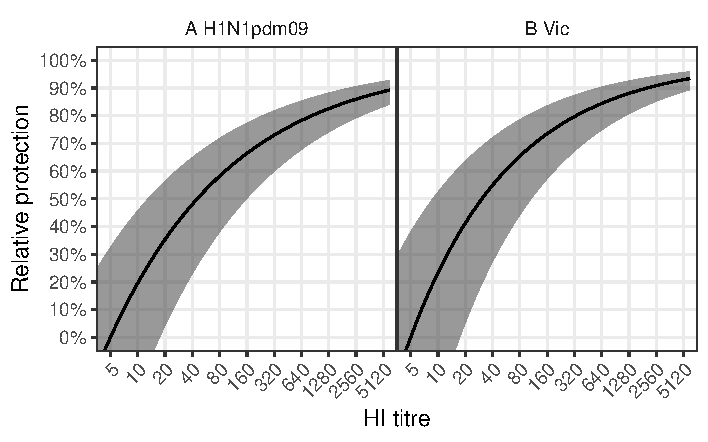
\includegraphics{../fit-cox-plot/sophia-og.pdf}
\caption{\label{fig:ogcurves}Published protection curves of Ng (2013)}
\end{figure}

\hypertarget{what-i-did}{%
\section{What I did}\label{what-i-did}}

I took the transformed data to be my starting point and I used the same model. This means that there are potentially questionable things that I did not question, these include:

\begin{itemize}
\item
  Extrapolation of flu proxy
\item
  Inclusion of flu proxy into the model
\item
  The waning titre model
\item
  Using a waning titre model with no account of censored observations
\end{itemize}

\pagebreak

\hypertarget{sec-problem}{%
\section{The problem with the original}\label{sec-problem}}

The code that generated one of the original curves is below (the same code generates the other curve, just with the variable names changed)

\begin{Shaded}
\begin{Highlighting}[]
\NormalTok{beta <-vic.vic}\OperatorTok{$}\NormalTok{coef}
\NormalTok{se <-}\KeywordTok{sqrt}\NormalTok{(}\KeywordTok{sum}\NormalTok{(}\KeywordTok{vcov}\NormalTok{(cox.td.B)))}
\NormalTok{est <-}\KeywordTok{data.frame}\NormalTok{(}\DataTypeTok{titer=}\KeywordTok{log2}\NormalTok{(}\DecValTok{5}\OperatorTok{*}\DecValTok{2}\OperatorTok{^}\NormalTok{(}\DecValTok{0}\OperatorTok{:}\DecValTok{9}\NormalTok{)),}\DataTypeTok{proxy=}\DecValTok{2}\NormalTok{, }\DataTypeTok{mu=}\OtherTok{NA}\NormalTok{, }\DataTypeTok{ci1=}\OtherTok{NA}\NormalTok{, }\DataTypeTok{ci2=}\OtherTok{NA}\NormalTok{)}
\NormalTok{est}\OperatorTok{$}\NormalTok{mu <-}\KeywordTok{exp}\NormalTok{(beta[}\DecValTok{1}\NormalTok{] }\OperatorTok{*}\StringTok{ }\NormalTok{est}\OperatorTok{$}\NormalTok{titer }\OperatorTok{+}\StringTok{ }\NormalTok{beta[}\DecValTok{2}\NormalTok{]}\OperatorTok{*}\NormalTok{est}\OperatorTok{$}\NormalTok{proxy  )}
\NormalTok{est}\OperatorTok{$}\NormalTok{ci1 <-}\KeywordTok{exp}\NormalTok{(beta[}\DecValTok{1}\NormalTok{] }\OperatorTok{*}\StringTok{ }\NormalTok{est}\OperatorTok{$}\NormalTok{titer }\OperatorTok{+}\StringTok{ }\NormalTok{beta[}\DecValTok{2}\NormalTok{]}\OperatorTok{*}\NormalTok{est}\OperatorTok{$}\NormalTok{proxy  }\OperatorTok{-}\StringTok{ }\FloatTok{1.96}\OperatorTok{*}\NormalTok{se)}
\NormalTok{est}\OperatorTok{$}\NormalTok{ci2 <-}\KeywordTok{exp}\NormalTok{(beta[}\DecValTok{1}\NormalTok{] }\OperatorTok{*}\StringTok{ }\NormalTok{est}\OperatorTok{$}\NormalTok{titer }\OperatorTok{+}\StringTok{ }\NormalTok{beta[}\DecValTok{2}\NormalTok{]}\OperatorTok{*}\NormalTok{est}\OperatorTok{$}\NormalTok{proxy }\OperatorTok{+}\StringTok{ }\FloatTok{1.96}\OperatorTok{*}\NormalTok{se)}
\NormalTok{est}\OperatorTok{$}\NormalTok{d <-(est}\OperatorTok{$}\NormalTok{mu[}\DecValTok{1}\NormalTok{]}\OperatorTok{-}\NormalTok{est}\OperatorTok{$}\NormalTok{mu)}\OperatorTok{/}\NormalTok{est}\OperatorTok{$}\NormalTok{mu[}\DecValTok{1}\NormalTok{]}
\NormalTok{est}\OperatorTok{$}\NormalTok{d.ci1 <-(est}\OperatorTok{$}\NormalTok{mu[}\DecValTok{1}\NormalTok{]}\OperatorTok{-}\NormalTok{est}\OperatorTok{$}\NormalTok{ci2)}\OperatorTok{/}\NormalTok{est}\OperatorTok{$}\NormalTok{mu[}\DecValTok{1}\NormalTok{]}
\NormalTok{est}\OperatorTok{$}\NormalTok{d.ci2 <-(est}\OperatorTok{$}\NormalTok{mu[}\DecValTok{1}\NormalTok{]}\OperatorTok{-}\NormalTok{est}\OperatorTok{$}\NormalTok{ci1)}\OperatorTok{/}\NormalTok{est}\OperatorTok{$}\NormalTok{mu[}\DecValTok{1}\NormalTok{]}
\end{Highlighting}
\end{Shaded}

The problem is this line

\begin{Shaded}
\begin{Highlighting}[]
\NormalTok{se <-}\KeywordTok{sqrt}\NormalTok{(}\KeywordTok{sum}\NormalTok{(}\KeywordTok{vcov}\NormalTok{(cox.td.B)))}
\end{Highlighting}
\end{Shaded}

It sets the standard error to a number (square root of the sum of entries in the variance-covariance matrix) which is used to generate the interval bounds across the entire covariate range.

The linear predictor \(l\) part of the model has this form

\[
l=\beta_TX_\text{logtitre}+\beta_PP
\]

What we want is the variance of \(l\) which is

\[
V(l)=X_\text{logtitre}^2V(\beta_T)+P^2V(\beta_P)+2X_\text{logtitre}P\ Cov(\beta_T,\beta_P)
\]

Which is only equal to the sum of entries of the variance-covarinace matrix when both \(X_\text{logtitre}\) and \(P\) are 1.

\hypertarget{correcting-confidence-intervals}{%
\section{Correcting confidence intervals}\label{correcting-confidence-intervals}}

The quantity that we are looking for is protection \(r\) which is

\[
r=1-\text{exp}(l)
\]

Note that the curves in Figure \ref{fig:ogcurves} are supposed to show protection relative to the titre of 5.

So then the target quantity is

\[
r=1-\text{exp}(\beta_T(X_\text{logtitre}-\text{log}(5))+\beta_PP)
\]

The code chunk in Section \ref{sec-problem} extracts this by doing this wierd manipulation

\begin{Shaded}
\begin{Highlighting}[]
\NormalTok{est}\OperatorTok{$}\NormalTok{d <-(est}\OperatorTok{$}\NormalTok{mu[}\DecValTok{1}\NormalTok{]}\OperatorTok{-}\NormalTok{est}\OperatorTok{$}\NormalTok{mu)}\OperatorTok{/}\NormalTok{est}\OperatorTok{$}\NormalTok{mu[}\DecValTok{1}\NormalTok{]}
\end{Highlighting}
\end{Shaded}

Which is

\[
\begin{aligned}
r &= \frac{\text{exp}(\beta_T\text{log}(5)+2\beta_P)-\text{exp}(\beta_TX_\text{logtitre}+2\beta_P)}{\text{exp}(\beta_T\text{log}(5)+2\beta_P)} \\
&=
1 - \text{exp}(\beta_T(X_\text{logtitre}-\text{log}(5)))
\end{aligned}
\]

Meaning \(P\) (flu proxy) is set to 0, so the variance of the linear part of this quantity is simply

\[
V(r^{linear})=(X_\text{logtitre}-\text{log}(5))^2V(\beta_T)
\]

So both the quantity and its correct variance could have been extracted from the model fit directly

\begin{Shaded}
\begin{Highlighting}[]
\NormalTok{est}\OperatorTok{$}\NormalTok{r_linear <-}\StringTok{ }\KeywordTok{coef}\NormalTok{(vic.vic)[[}\DecValTok{1}\NormalTok{]] }\OperatorTok{*}\StringTok{ }\NormalTok{(est}\OperatorTok{$}\NormalTok{titer }\OperatorTok{-}\StringTok{ }\KeywordTok{log2}\NormalTok{(}\DecValTok{5}\NormalTok{))}
\NormalTok{est}\OperatorTok{$}\NormalTok{r_var <-}\StringTok{ }\NormalTok{(est}\OperatorTok{$}\NormalTok{titer }\OperatorTok{-}\StringTok{ }\KeywordTok{log2}\NormalTok{(}\DecValTok{5}\NormalTok{))}\OperatorTok{^}\DecValTok{2} \OperatorTok{*}\StringTok{ }\KeywordTok{vcov}\NormalTok{(vic.vic)[}\DecValTok{1}\NormalTok{, }\DecValTok{1}\NormalTok{]}
\end{Highlighting}
\end{Shaded}

And then used to generate probability-scale quantities

\begin{Shaded}
\begin{Highlighting}[]
\NormalTok{est}\OperatorTok{$}\NormalTok{d <-}\StringTok{ }\DecValTok{1} \OperatorTok{-}\StringTok{ }\KeywordTok{exp}\NormalTok{(est}\OperatorTok{$}\NormalTok{r_linear)}
\NormalTok{est}\OperatorTok{$}\NormalTok{d.ci1 <-}\StringTok{ }\DecValTok{1} \OperatorTok{-}\StringTok{ }\KeywordTok{exp}\NormalTok{(est}\OperatorTok{$}\NormalTok{r_linear }\OperatorTok{+}\StringTok{ }\KeywordTok{qnorm}\NormalTok{(}\FloatTok{0.975}\NormalTok{) }\OperatorTok{*}\StringTok{ }\KeywordTok{sqrt}\NormalTok{(est}\OperatorTok{$}\NormalTok{r_var))}
\NormalTok{est}\OperatorTok{$}\NormalTok{d.ci2 <-}\StringTok{ }\DecValTok{1} \OperatorTok{-}\StringTok{ }\KeywordTok{exp}\NormalTok{(est}\OperatorTok{$}\NormalTok{r_linear }\OperatorTok{-}\StringTok{ }\KeywordTok{qnorm}\NormalTok{(}\FloatTok{0.975}\NormalTok{) }\OperatorTok{*}\StringTok{ }\KeywordTok{sqrt}\NormalTok{(est}\OperatorTok{$}\NormalTok{r_var))}
\end{Highlighting}
\end{Shaded}

The curves that result from this correction are in Figure \ref{fig:cicurves}

\begin{figure}
\centering
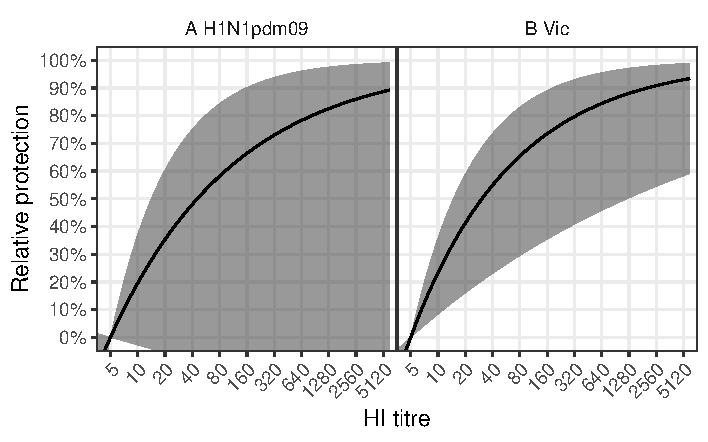
\includegraphics{../fit-cox-plot/sophia-ci.pdf}
\caption{\label{fig:cicurves}Ng (2013) curves but with corrected CIs}
\end{figure}

\pagebreak

\hypertarget{correcting-model-fit}{%
\section{Correcting model fit}\label{correcting-model-fit}}

There is another problem with the above intervals which is how the model was fit.

\begin{Shaded}
\begin{Highlighting}[]
\NormalTok{vic.vic<-cox.td.B <-}\StringTok{ }\KeywordTok{coxph}\NormalTok{(}\KeywordTok{Surv}\NormalTok{(t,event)}\OperatorTok{~}\NormalTok{postvax.b}\OperatorTok{+}\NormalTok{proxy,}\DataTypeTok{data=}\NormalTok{kdata.td.b)}
\end{Highlighting}
\end{Shaded}

This assumes that every row from the dataset is an independent right-censored observation. There are 773 observations in \texttt{kdata.td.b} but 244,382 rows. So fitting a model like this implies that we have 244,382 subjects in the study who we followed anywhere from 0 to 413 days.

To fit this properly we need to create the start and the end timepoints for each row and cluster on individual id.

\begin{Shaded}
\begin{Highlighting}[]
\KeywordTok{library}\NormalTok{(dplyr)}
\NormalTok{kdata.td.b <-}\StringTok{ }\NormalTok{kdata.td.b }\OperatorTok
\StringTok{  }\KeywordTok{group_by}\NormalTok{(hhid) }\OperatorTok
\StringTok{  }\KeywordTok{mutate}\NormalTok{(}
    \DataTypeTok{start =}\NormalTok{ t,}
    \DataTypeTok{end =} \KeywordTok{lead}\NormalTok{(t, }\DataTypeTok{default =} \KeywordTok{max}\NormalTok{(t) }\OperatorTok{+}\StringTok{ }\DecValTok{1}\NormalTok{)}
\NormalTok{  ) }\OperatorTok
\StringTok{  }\KeywordTok{ungroup}\NormalTok{()}
\NormalTok{vic.vic <-}\StringTok{ }\KeywordTok{coxph}\NormalTok{(}
  \KeywordTok{Surv}\NormalTok{(start, end, event) }\OperatorTok{~}\StringTok{ }\NormalTok{postvax.b }\OperatorTok{+}\StringTok{ }\NormalTok{proxy }\OperatorTok{+}\StringTok{ }\KeywordTok{cluster}\NormalTok{(hhID),}
  \DataTypeTok{data =}\NormalTok{ kdata.td.b}
\NormalTok{)}
\end{Highlighting}
\end{Shaded}

The protection curves that result from the corrected model call and the corrected intervals are in Figure \ref{fig:cimodcurves}.

\begin{figure}
\centering
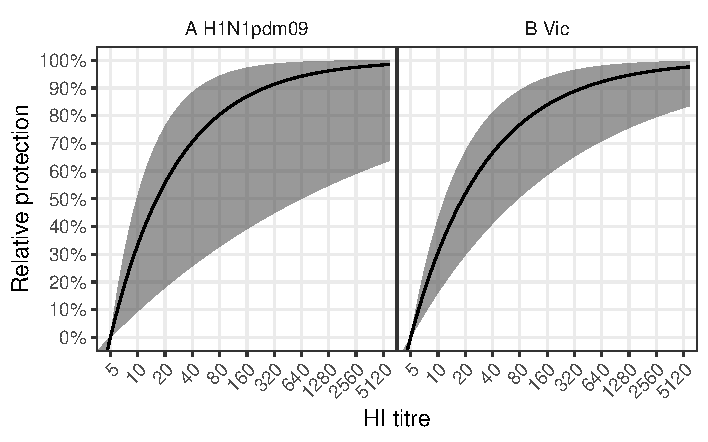
\includegraphics{../fit-cox-plot/sophia-ci-mod.pdf}
\caption{\label{fig:cimodcurves}Ng (2013) curves with corrected fit and CIs}
\end{figure}

The curves I generated by fitting a simple one-covariate one-row-per-observation right-censored Cox model with no proxy or waning titres are in Figure \ref{fig:mycurves}. They look remarkably similar to Figure \ref{fig:cimodcurves}.

\begin{figure}
\centering
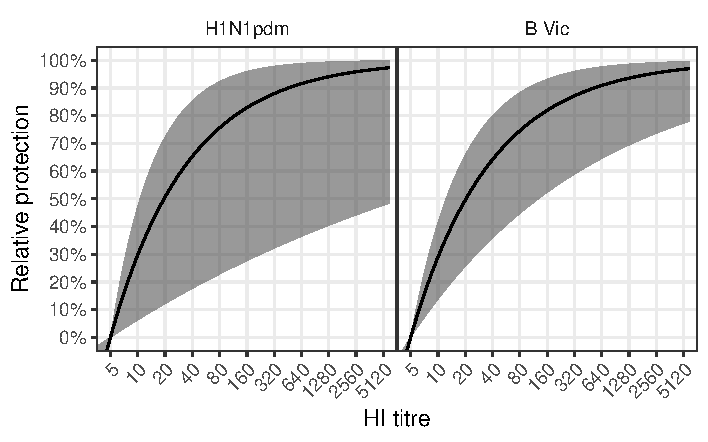
\includegraphics{../fit-cox-plot/kiddyvaxmain.pdf}
\caption{\label{fig:mycurves}Protection curves from simple one-covariate one-row-per-observation right-censored Cox model with no proxy or waning titres}
\end{figure}

\end{document}
